\chapter{Data Aggregation With Internal Verification} % (folit
\label{cha:Data Aggregation With Internal Verification}

% \section{System Design importantplementations}
	The high level idea of the aggregate commit with verification scheme is that all the sensor nodes in the network send the signature of the message along with the message.
	They send their certificates if the parent node does not have it already.
	The parent node verifies all the received signatures from its children.
	And proceeds with the aggregation process.
	After aggregation, the parent node can throw away all the signatures from its children and signs the message of its children or it can pass its children's signatures to its parent. 
	The pros and cons of each approach are discussed in the following sections. 
	And once the base station receives the aggregated value it starts the verification process. 
	If there is no malicious activity in the network then  it accepts the result and takes an action.
	If the malicious activity is detected during the verification phase then the base station starts interactive activity to detect an adversary. 

\section{Data-Item}
	
	We describe structure of the data-item and its signature, used in creating the commitment tree for the aggregate commit with verification approach. And differences between the data-item and the label structure of SHIA, with rational behind it.
	\begin{definition}
		\label{def:data-item}
		A commitment tree is a binary tree where each vertex has an associated data-item representing the data that is passed on to its parent. The data-items have the following format:

		$\hspace{100pt}$ \textbf{$<\ $id, count, value, commitment$\ >$}\\
	Where $id$ is the unique ID of the node; $count$ is the number of leaf vertices in the subtree rooted at this vertex; $value$ is the SUM aggregate computed over all the leaves in the subtree and $commitment$ is a cryptographic commitment.
	\end{definition}
	Each sensor node creates its own data-item during commitment tree generation process which is called the leaf vertex of the node.
	For example, sensor node $S$ creates its data-item $S_{0}$ as follows:
	\begin{equation}
		\label{eq:data-item}
	 	S_{0} =\ <S_{id}, 1, S_{value}, H(N||1||S_{value})>
	 \end{equation}
	where $S_{id}, S_{value}$ is the unique ID and sensor reading of the sensor node $S$. 
	The count is $1$ as there is only vertex in the subtree rooted at $S$, $H$ is the collision resistant hash function, and $N$ is the query nonce.

	The first difference between SHIA's label structure and our data-item structure is that we remove the $complement$ field from the label structure Defined \ref{def:label}. 
	We think the complement filed is redundant information in the label. 
	The complement field is used by the base station (the querier, according to SHIA), before the result checking phase, to verify \textbf{SUM + COMPLEMENT =} $\textbf{n} \cdot \textbf{r}$ ; where $\textbf{n}$ is the number of nodes in the network, $\textbf{r}$ is the upper bound on the allowed sensor readings.
	We can achieve the same upper bound without the complement field.
	As the querier knows $n, r$ and it gets SUM from the root of the aggregation tree.
	If \textbf{SUM} $> \textbf{n} \cdot \textbf{r}$ , then the base station knows some node or nodes in the network reported out of range readings.

	The second difference between SHIA's label structure and our data-item structure is that we include unique ID of the node in its data-item.
	SHIA does not have the ID field in their label structure as they do not do internal verification while creating a commitment tree and while distributing off-path values.
	Also, in the label format ID of the node is hashed in the commitment field after the first aggregation and virtually gets lost.
	Hence, SHIA can not provide security services such as authenticity, non-repudiation and is vulnerable to all sorts of active attacks.
	We do internal verification while creating the commitment tree and distributing off-path values.
	So, it is necessary for any aggregate node to know the ID of all the received data-items in its forest, for the verification of the received signatures as shown in the following sections.

	\subsection{Signing and Verification of the Data-Item}
		\label{subsection:Signing and Verification of the Data-Item}
		Each sensor node sends the signature of its data-item signed by itself using its own secret key. 
		For example, the signature of $S_{0}$ of the Equation \ref{eq:data-item} is given as follows:
		\begin{equation}
			\label{eq:sign-data-item}
			\textsf{S} = \textsf{Sign}_{S_{S}}(S_{0})
		\end{equation}
		where $S_{S}$ is the secret key of the sensor node $S$, $\textsf{Sign}$ is the signing algorithm.
		The parent node receives the data-item and its signature from its child. 
		It also receives the certificate from its child which is shown in Table \ref{table:digital-certificate}.
		\begin{table}[!htb]	
			\begin{center}
				\begin{tabular}{ |l| }
			    \hline
			    Unique ID of the sensor node \\
			    \hline
			    Public key of the sensor node \\	
			    \hline
			    Certification Authority's name \\
			    \hline
			    Certification Authority's digital signature \\
			    \hline
				\end{tabular}
			\end{center}
	  	\caption{Digital Certificate}
		  \label{table:digital-certificate}
	  \end{table}
	  From the digital certificate the parent node receives the public-key of its child, which is necessary to verify the signature.
	  For example, the parent node of $S$ verifies $\textsf{Sign}_{S_{S}}(S_{0})$ as follows:
	  \begin{equation}
			\textsf{Verify}_{P_{S}}(S_{0},\textsf{S}) = 
			\begin{cases}
			 \textbf{true}\ \mbox{with probability of 1} & if\ \textsf{S} = \textsf{Sign}_{S_{S}}(S_{0})\\
			 \textbf{false}\ \mbox{with overwhelming probability} & if\ \textsf{S} \neq \textsf{Sign}_{S_{S}}(S_{0})
			\end{cases}
			\label{eq:verification}
		\end{equation}
	  where $P_{S}$ is the public key of $S$, $\textsf{Verify}$ is the verification algorithm.
	
	\subsection{Security Benefits}
		\label{subsec:security benefits of signing the data-item}
		% \textcolor{red}{remove payload}
		While creating the commitment tree, the sensor $S$ sends the data-item $S_{0}$, and its signature $\textsf{S}$ to its parent in the aggregation tree.
		The signature allows the parent node to verify the \textit{authenticity} of the sensor node.
		As only sensor node $S$ can create the signature using its secret key. 
		The signature $\textsf{S}$ assures the \textit{integrity} of the data-item $S_{0}$.
		Because either the data-item or the signature has been tampered in any way the verification algorithm return false.
		Furthermore, it allows the sender to have the proof for the sent data-item.
		And the receiver for the proof for the received data-item, providing the security service of \textit{non-repudiation}.
		The digital signature depends on the message so the parent node can not reuse the signature for other data-items in the future.
		Hence, protecting the network against the \textit{replay attacks}.
		Hence, it protects against the \textit{active attacks}.

\section{Commitment Payload}

	We define commitment payload based on the commitment forest Defined in \ref{def:commitment-forest}.
	We also define transmit payload as follows.
	\begin{definition}
		A \textbf{commitment payload} is a set of data-items of the root vertices of the trees with their respective signatures in the outgoing commitment forest and an additional signature for the transmission.
	\end{definition}
	\begin{definition}
		A \textbf{transmit payload} is the concatenation of all the data-items in the commitment payload.
	\end{definition}
	% We use the term payload for commitment payload and the term forest for the commitment forest.
	For brevity, we use the term forest, payload instead of commitment forest, commitment payload respectively.
	Consider, the aggregation tree shown in Figure \ref{fig:Palm aggregation tree}, where $B$ is the parent of $A$, $C$ is the parent of $B$ and $D$ is the parent of $C$. 
	\begin{figure}[h!]
		\centering
		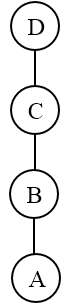
\includegraphics[scale = 1]{images/palm-aggregation-tree.png}
		\caption{Palm Shaped Aggregation Tree}
		\label{fig:Palm aggregation tree}
	\end{figure}
	While creating the commitment tree $A$ creates its data-item $A_{0}$ according to Equation \ref{eq:data-item}.
	$A$ sends only one data-item to $B$ therefore $A$'s transmit-payload ($A_{\tau}$), the payload($A_{p}$) are given as follows:
	\begin{equation}
		\label{eq:signing-payload}
			A_{p} =\ <A_{0}, \textsf{Sign}_{S_{A}}(A_{0}), \textsf{Sign}_{S_{A}}(A_{\tau}) >\ where\ A_{\tau} =\ < A_{0} > 
	\end{equation}
	The sensor node $C$'s payload is shown in Figure \ref{fig:Commitment payload of C}.
	The commitment tree generation process is described in the later sections. 
	The sensor node $C$ sends two data-items to $D$ therefore $C$'s transmit-payload($C_{\tau}$), the payload($C_{p}$) are given as follows:
	\begin{equation}
		 	C_{p} =\ <C_{0}, \textsf{Sign}_{S_{C}}(C_{0}), B_{1}, \textsf{Sign}_{S_{C}}(B_{1}), \textsf{Sign}_{S_{C}}(C_{\tau}) >\ where\ C_{\tau} =\ <B_{1}\ ||\ C_{0}>
	\end{equation}
	\begin{figure}[h!]
		\centering
		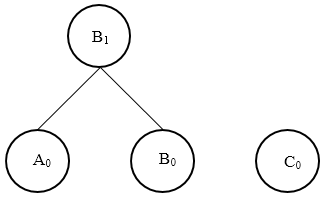
\includegraphics[scale = 1]{images/commitment-payload-of-C.png}
		\caption{Commitment Payload of Sensor Node $C$}
		\label{fig:Commitment payload of C}
	\end{figure}
	The verification of the received signatures of the payload is done by the parent node in the same way described in Section \ref{subsection:Signing and Verification of the Data-Item}.

	\subsection{Security Benefits}
		\textcolor{red}{Might need refactoring}
		As described in Subsection \ref{subsec:security benefits of signing the data-item}, the signature of the payload $\textsf{Sign}_{S_{S}}(S_{p})$ assures the integrity and authentication of the payload $S_{p}$.
		In addition to that, the signature of the payload is like the signature for the transmission.
		To the sender, it assures that it is sending only the data-items included in the signature of the payload.
		And none of the data-items gets added or remove from the payload during the transmission. 
		To the receiver, it assures that it receives all the data-items included in the signature of the payload. 
		And none of the data-items were stranded or added additionally to the payload of its child.
		For example, the signature on the $C$'s payload $\textsf{Sign}_{S_{C}}(C_{p})$ assures that the sensor node $C$ sent only two data-items $C_{0},B_{1}$ in its payload.
		And none of the data-items in its payload have been left stranded.
		It is true for the sensor node $A$.
		As we said, it like the signature for the transmission.

\section{Key Differences from SHIA}

	In SHIA, all the leaf nodes in the aggregation tree send only their respective data-items to the parent in the aggregation tree.
	In our approach, all the leaf nodes send the data-item, the signature of the data-item and the signature of the payload to their parent node in the aggregation tree. 
	The child node sends its certificate as well if the parent node does not have it in its memory already.

	In SHIA, the parent node proceeds with the aggregation process without verifying the received data-items.
	\textbf{The parent node first verifies the payload signature.}
	In our protocol, the parent node verifies the received signature using the the verification algorithm.
	And the parent node proceeds with the aggregation only if all the signatures were verified successfully.

	In SHIA, the trusted base station verifies the final received data-items.
	And upon detecting the malicious activity in the network, the base station raises an alarm. 
	The base station does not do anything to detect malicious node responsible for the malicious activity.
	In our approach, upon detecting the malicious activity the base station interacts with different nodes in the network to detect the malicious node.
	Also, the  base station issues the certificate to the sensor nodes in the network.
	
	\subsection{Bandwidth Analysis}
	
		\textcolor{red}{Might need refactoring}
		Typical size of the data-item packet is $400$ bits.
		If one uses Elliptic Curve Digital Signature Algorithm (ECDSA) then the size of signature is $500$ bits \cite{ecdsa2009186}.
		And the certificate size is $1500$ bits.
		So, at max we have to send additional $2000$ bits with the data-item.
		We think it is worthwhile to send these additional bits.
		Because of all the security benefits we gain from it. 
		\textbf{Note:} The packets size are close approximate to the actual packet size. 
		The actual packet size may differ based on the implementation.

\section{Two ways of Forwarding the Commitment Payload}	
	
	As described in the previous sections, we send the data-items with their signature along with the signature of the payload while creating the commitment tree.
	Here, we describe two different approaches to send the signatures in the aggregation tree hierarchy based on the two different ways of signing the data-items.
	To demonstrate two approaches we use the aggregation tree shown in Figure \ref{fig:Palm aggregation tree} and the payload of the sensor node $C$ shown in Figure \ref{fig:Commitment payload of C}.
	In both the approaches, the sensor node $C$ sends all the data-items in its payload with their respective signatures to its parent sensor node $D$ along with the signature of its payload $C_{p}$.

	In the first approach, $C$ verifies $\textsf{Sign}_{S_{B}}(B_{1})$ and sends it to $D$ without any modifications as follows:
	\begin{equation}	
		\begin{array}{l}
			C_{p} =\ <C_{0},\textsf{Sign}_{S_{C}}(C_{0}),B_{1},\textcolor{red}{\textsf{Sign}_{S_{B}}(B_{1})}, \textsf{Sign}_{S_{C}}(C_{\tau})>\ where\ C_{\tau} = <C_{0} || B_{1}>\\
			C_{0} =\ <C_{id}, 1, C_{value}, H(N||1||C_{value})>\\
			B_{1} =\ <B_{id}, 2, B_{1value}, H(N||2||B_{1value}||A_{0}||B_{0})>\\
		\end{array}
		\label{eq:forwarding-payload-without-resigning}
	\end{equation}
	% The sensor node $C$ has two data-items $C_{0},B_{1}$ in its payload. 
	The sensor node $C$ sends three signatures $\textsf{Sign}_{S_{B}}(B_{1})$, $\textsf{Sign}_{S_{C}}(C_{0}) $ and $\textsf{Sign}_{S_{C}}(C_{p})$ to its parent $D$.
	It requires the parent node $D$ to know the public key of the sensor nodes $C$ and $B$, hence two certificates.

	In the second approach, the sensor node $C$ can verify the $\textsf{Sign}_{S_{B}}(B_{1})$ then remove the old signature and creates new signature $\textsf{Sign}_{S_{C}}(B_{1})$ and sends to $D$ as follows:
	\begin{equation}	
		\begin{array}{l}
			C_{p} =\ <C_{0},\textsf{Sign}_{S_{C}}(C_{0}),B_{1},\textcolor{red}{\textsf{Sign}_{S_{C}}(B_{1})}, \textsf{Sign}_{S_{C}}(C_{\tau})>\ where\ C_{\tau} = <C_{0} || B_{1}>\\
			C_{0} =\ <C_{id}, 1, C_{value}, H(N||1||C_{value})>\\
			B_{1} =\ <B_{id}, 2, B_{1value}, H(N||2||B_{1value}||A_{0}||B_{0})>\\
		\end{array}
		\label{eq:forwarding-payload-with-resigning}
	\end{equation}
	The sensor node $C$ sends three signatures $\textsf{Sign}_{S_{C}}(B_{1})$, $\textsf{Sign}_{S_{C}}(C_{0}) $ and $\textsf{Sign}_{S_{C}}(C_{p})$ to its parent $D$.
	But all the signatures are signed by the sensor node $C$, it requires the parent node $D$ to know the public key of only the sensor node $C$, hence $D$ need to know only one certificate.

	To give an analogy with the real world application consider the following example.
	One want to buy a diamond from the local diamond retailer.
	Diamond is an expensive commodity so the end customer wants to verify its authenticity and integrity before purchasing.
	Suppose, the diamond was created by the manufacturer in Africa, it was sold to a national wholesaler in the United States. 
	The national wholesaler sells it to the state level reseller and he sells it to the city or county level retailer from whom the customer purchases the diamond.

	One approach to verify the authenticity of the commodity is to make each entity in the supply chain to verify all the signatures on the received entity and sign on top of it.
	And then forward the commodity with all the signatures to the next entity in the supply chain.
	The next entity repeats the same procedure.
	Hence, any entity in the supply chain need to verify the signatures of all its descendants in the supply chain.
	In our example, it means to make the manufacturer from Africa signs the diamond and sells the signed diamond with his certificate to the national level wholesaler in United States.
	The national level wholesaler in United States verifies the signature from the manufacturer using manufacturer's certificate.
	Then he adds his signature and certificate, and sells the diamond signed with two signatures and two certificates to the state level reseller.
	The state level reseller verifies both the signatures on the diamond using the respective certificates.
	Then he adds his signature and certificate, and sells the diamond singed with three signatures and three certificates to the city level retailer. 
	The city level retailer does the same thing before selling the diamond to the end customer.
	In the end, the customer needs to verify all four signatures, using the respective certificates.

	% Note: that the same diamond now has been signed by four different entities. And the end customer need to know the certificate of all four parties to verify all those signatures.

	An alternative approach to verify the authenticity of the commodity is to make each entity in the supply chain verify the signature, throw away the old signature, and then add its own signature on it. 
	It means the next entity in the supply chain need to verify only a single signature.
	The next entity repeats the same procedure.
	Hence, any entity in the supply chain need to verify the signature of only its direct peer in the supply chain. 
	In our example, it means to make the manufacturer from Africa signs the diamond and sells the signed diamond with his certificate to the national level wholesaler in United States.
	The national level wholesaler in United States verifies the signature from the manufacturer using the manufacturer's certificate.
	Then he removes the signature of the manufacturer, adds his own signature and certificate, and sells the diamond signed with one signature and one certificate to the state level reseller.
	The state level reseller verifies only the signature from the wholesaler using the wholesaler's certificate.
	Then he removes the signature of the wholesaler, adds his own signature and certificate, and sells the diamond signed with one signature and one certificate to the city level retailer.
	The city level retailer does the same thing before selling the diamond to the end customer.
	In the end, the customer needs to verify only one signature of the city level retailer using retailer's certificate.
	This approach requires very few number of certificates overall in the supply chain.

	We call these two approaches \textbf{Forwarding signatures without resigning the data-items}, \textbf{Forwarding signatures with resigning the data-items} as shown in Equations \ref{eq:forwarding-payload-without-resigning} and \ref{eq:forwarding-payload-with-resigning} respectively.
	Both the approaches have their pros and cons and the perfect approach depends heavily on the application.
	The various aspects of both the approaches for sensor nodes are discussed in the following sections.

	\section{Comparison of two approaches for forwarding the Commitment Payload}
		To do the analysis we developed a performance matrix. 
		We analysis different network topologies based on that matrix.
		% In both the approaches, the commitment tree is complete binary.
		% As we know, the complete binary tree has  $2^{h + 1} - 1$ vertices in the tree; where $h$ is the height of the tree with the root height is $0$. 
		% So, we need $\Omega(2^{h + 1} - 1)$ signatures in both the approaches. 
		% Analysis model:	
		% 	While creating CT;While distributing off-path; Both places together\\
		% Initial analysis says, if a single aggregate node cheats while CT generation or distributing off-path values it gets caught.

		Table \ref{table:Analysis table for Star Aggregation Tree} shows the analysis for the star tree network with $n$ nodes while creating the commitment tree.
		\begin{table}[!htb]	
			\begin{center}
				\begin{tabular}{ |l| l| l| }
			    \hline
			    & With resigning & Without resigning \\
			    \hline
			    Number of created signatures & $2n + 1$ & $2n + 1$ \\	
			    \hline
			    Number of transmitted signatures & T & T\\
			    \hline
			    Number of signing activity & $2n + 1$ & $2n + 1$ \\
			    \hline
			    Number of verifying activity & $n - 1$ & $n - 1$ \\
			    \hline
			    Number of certificates & $n - 1$ & $n - 1$ \\
			    \hline
			    Edge congestion & $3(n - 1)$ & $3(n - 1)$\\
			    \hline
				\end{tabular}
			\end{center}
	  	\caption{Analysis for Star Aggregation Tree}
		  \label{table:Analysis table for Star Aggregation Tree}
	  \end{table}

	  Table \ref{table:Analysis table for Palm Aggregation Tree} shows the analysis for the star tree network with $n$ nodes while creating the commitment tree.
		\begin{table}[!htb]	
			\begin{center}
				\begin{tabular}{ |l| l| l| }
			    \hline
			    & With resigning & Without resigning \\
			    \hline
			    Number of created signatures & T & $2n$ \\	
			    \hline
			    Number of transmitted signatures & T & T\\
			    \hline
			    Number of signing activity & T & T \\
			    \hline
			    Number of verifying activity & T & T \\
			    \hline
			    Number of certificates & T & T \\
			    \hline
			    Edge congestion & T & T\\
			    \hline
				\end{tabular}
			\end{center}
	  	\caption{Analysis for Palm Aggregation Tree}
		  \label{table:Analysis table for Palm Aggregation Tree}
	  \end{table} 
		
		Note that we send signatures while distributing off-path values as well.
	
		If we throw away the old signatures and resign the data-item with current aggregate node then following is true:
			\begin{itemize}
				\item Each parent needs the certificates of only its direct children.
				\item Each child needs to know the certificate of its parent only.
				\item Number of signatures remain the same as previous approach.
				\item Number of certificates needed in the network is $O(n)$; n is the number of nodes in the network.
				\item We do not need the signature of the payload.
			\end{itemize}

	\section{\textcolor{red}{Forwarding signatures without resigning the data-items}}
